\section{Backend de la solución}

La solución almacena información detallada acerca de las acciones del usuario,
las condiciones de estas acciones y el contexto en el cual fueron ejecutadas.

Esta información es almacenada en un servidor dedicado para su posterior
análisis.

\begin{figure}[ht]
\centering
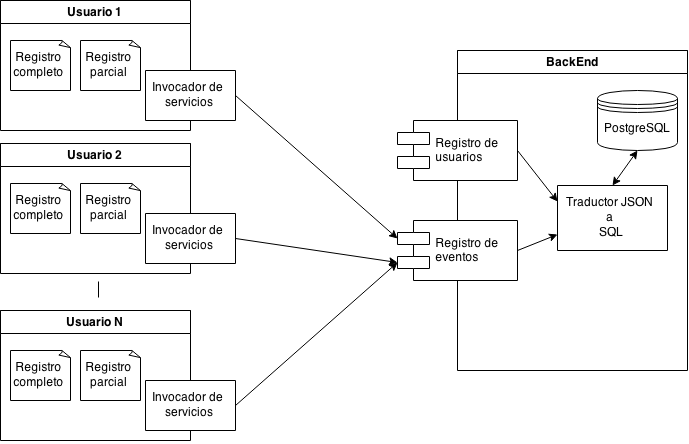
\includegraphics[scale=0.5]{propuesta/backend_diagrama.png}
\caption{Diagrama de la interacción de los usuarios con el \textit{BackEnd}, se
    puede observar a grandes rasgos, los componentes del sistema y los servicios
    que ofrece.}
\label{fig:backend_diagrama}
\end{figure}

En la figura~\ref{fig:backend_diagrama} se pueden observar los componentes
principales de este sistema, y su interacción con los dispositivos móviles de
los usuarios. 

\subsection{Registro de usuarios}

Para poder determinar a qué usuario corresponde qué conjunto de datos, durante la
instalación de la solución en los dispositivos móviles de los usuarios, se ingresa como
un dato adicional el número de teléfono del mismo, estos datos se registran
en el \textit{BackEnd} al mismo tiempo en el que se muestra la solución al usuario.

De esta forma, en el sistema se encuentran los datos proveídos por la
simulación, así como el nombre del usuario. Es necesario almacenar el nombre del
usuario para las diversas encuestas que se realizan (las encuestas para alumnos
que participaron en el experimento no son anónimas), de esta manera se puede
saber, dada una encuesta, a que alumno corresponde y el uso que le dio a la
solución. Estas encuestas son explicadas en detalle en \ref{chap:evaluacion} y sus 
resultados en \ref{chap:analisis}.

\subsection{Registro de eventos}

Las acciones que realiza el usuario son almacenadas en un archivo temporal,
dentro del dispositivo móvil del usuario, cuando este decide enviar la
información, estos datos se transmiten por la red a un servidor que almacena el
\textit{BackEnd}.

Una vez que el usuario envía sus datos de uso, el archivo de registros
local se limpia, permitiendo así que nuevos registros sean añadidos.
Adicionalmente, existe un archivo de respaldo, que contiene toda la información
que se registró del usuario, incluyendo aquellas que ya fueron enviadas al
servidor \textit{BackEnd}.

\subsection{Detalles de implementación}

El \textit{BackEnd} es un sistema web, desarrollado en \textit{Java}, y
desplegado en un servicio \textit{OpenShift}, el cual está disponible $24$ horas
al día, los $7$ días a la semana, asegurando así, que cuando el usuario desee
enviar datos lo pueda hacer sin problemas.

El sistema tiene dos servicios web que permiten el registro de usuarios y el
registro de eventos, ambos reciben una lista de elementos y los almacenan en una
base de datos \textit{PostgreSQL}.

Estos dos servicios implementan un mecanismo de seguridad sencillo, basado en usuario y
contraseña, el único objetivo de este mecanismo, es que los datos no sean
fácilmente accesibles, pues contienen datos sensibles.

La petición enviada desde la solución, contiene el número de teléfono del
usuario, un identificador único generado por \textit{Unity3D} y una lista de
eventos, en formato \Gls{json}.

